\documentclass[a4paper,11pt]{article}
\usepackage[margin=1in]{geometry}
\usepackage[T1]{fontenc}
\usepackage{lmodern}
\usepackage{amsmath,amssymb,amsthm,graphicx,booktabs}
\newcommand{\norm}[1]{\left\|#1\right\|}
\newcommand{\inner}[2]{\left\langle#1,#2\right\rangle}
\newcommand{\R}{\mathbb R}
\newcommand{\ceil}[1]{\left\lceil#1\right\rceil}
\DeclareMathOperator{\artanh}{artanh}
\setlength{\emergencystretch}{3em}
\usepackage[hidelinks]{hyperref}
\hypersetup{pdftitle={Sharp Error Bounds and Adaptive Stopping for Frank-Wolfe beyond Convexity},pdfauthor={Yaroslav P. Lyakhov and Stepan A. Suvorov}}
\newtheorem{theorem}{Theorem}[section]
\newtheorem{lemma}[theorem]{Lemma}
\newtheorem{proposition}[theorem]{Proposition}
\newtheorem{corollary}[theorem]{Corollary}
\newtheorem{example}[theorem]{Example}
\title{Sharp Error Bounds and Adaptive Stopping\\for Frank-Wolfe beyond Convexity}
\author{Yaroslav P. Lyakhov \and Stepan A. Suvorov}
\date{12 November 2026}
\begin{document}
\maketitle
\begin{abstract}
Under shifted restricted secant regularity and an affine loss-dependent
Hessian-norm bound, we derive sharp global-error certificates from the
full Frank-Wolfe gap, gradient norm and domain diameter. A constrained
minimizer may have a nonzero gradient. One radial comparison yields
the separate and joint envelopes; smooth examples approach them with
the observations and diameter fixed exactly whenever feasible. We characterize when the
ordinary gap already bounds the error. In that regime, the joint
certificate needs one scalar equation or admits an algebraic upper
bound; otherwise a finite grid gives certified enclosures. A nonlinear
calibration theorem supplies stopping bounds with adaptive directional
accuracy, counting failed refinements, rejected objective trials and
the terminal query. It covers away steps and finite-variance
median-of-means observations under exact objective values. Realizable
sigmoid regression provides a nonconvex application with explicit
constants. Fixed scalar checks verify the formulas and implementation.
\end{abstract}

\section{Introduction}
Frank-Wolfe methods replace projection by linear minimization over a
compact convex set. For a convex objective, their full gap bounds the
global error. For a nonconvex objective, a small gap usually certifies
only stationarity. A global stopping rule therefore needs a quantitative
relation between the observations and the error.

We study this relation under shifted restricted secant regularity and
the loss-dependent curvature bound
\[
 \|\nabla^2 f(x)\|\le H_0+H_1\bigl(f(x)-f(x^*)\bigr).
\]
The minimizer can lie on the boundary and have a nonzero gradient.
The Hessian norm is not squared. This model, used in the analysis of
warm-up \cite{warmup}, differs from curvature controlled by
$L_0+L_1\|\nabla f(x)\|$, as studied for Frank-Wolfe in
\cite{vyguzov}. Fixed-center regularity and restricted secant
conditions are established alternatives to convexity
\cite{regregularity,rsipep}.

The main result is a sharp bound on the error from the full gap $g$,
the gradient norm $P$, and optionally the diameter $D$. A single radial
comparison yields the separate norm and gap envelopes and the joint
envelopes $\mathcal J(g,P)$ and $\mathcal J_D(g,P)$. Their sharpness
holds over functions and domains satisfying the assumptions, even when
both observations and the diameter are prescribed exactly; positive
exact observations are feasible precisely when $g\le PD$. It does not
claim sharpness for each fixed domain.

We also determine exactly when the ordinary gap itself bounds the error.
The criterion needs arithmetic and a square root. Within that regime,
the joint envelope reduces to one scalar equation; an algebraic upper
bound avoids even that solve. Outside it, a finite grid and scalar
bisection give certified enclosures with explicit comparison budgets.
The radius profile need not be concave. The global enclosure assumes
neither concavity nor unimodality.

A second result turns any suitable nonlinear gap calibration into a
stopping rule with adaptive directional accuracy. The count includes
failed accuracy checks, rejected objective trials, and the final query.
It extends to away steps and to median-of-means directional estimates
with one confidence event for all adaptively requested queries.
The iteration uses the established backtracking rule
\cite{pedregosa,lacostejaggi}; the contribution concerns its certificates
and complete work accounting. Relative-error first-order oracles and
adaptive Frank-Wolfe variants are also studied in
\cite{oraclehallak,oracledenisov}.

The paper ends with explicit constants for realizable sigmoid regression
on an $\ell_1$ ball and fixed checks of the certificate formulas.
The certificates proved here do not by themselves establish a runtime
improvement.

\section{Model and radial reduction}
\label{compact:assumptions}\label{sec:model}
Let $Q\subset\mathbb R^d$ be a nontrivial compact convex set, let
$f$ be $C^2$ on a neighborhood of $Q$, and fix $x^*\in\arg\min_Q f$.
Write
\[
 \delta(x)=f(x)-f(x^*),\qquad
 P(x)=\|\nabla f(x)\|.
\]
\begin{equation}\label{eq:gap}
 G(x)=\max_{v\in Q}\langle\nabla f(x),x-v\rangle.
\end{equation}
The full Frank-Wolfe gap $G$ uses all of $Q$. Throughout the certificate
sections, the supplied constants satisfy $m>0$, $H_0,H_1\ge0$, and
\begin{equation}\label{boundarygap:assumptions}
 \begin{aligned}
 \langle\nabla f(z)-\nabla f(x^*),z-x^*\rangle
   &\ge m\|z-x^*\|^2,\\
 \|\nabla^2 f(z)\|&\le H_0+H_1\delta(z),\qquad z\in Q.
 \end{aligned}
\end{equation}
The first inequality is shifted restricted secant regularity (RSI).
Neither convexity of $f$ nor $\nabla f(x^*)=0$ is assumed.
The norm results below only require that $Q$ contain every segment
$[x^*,x]$, with $f$ smooth near those segments.

For $x\ne x^*$, set $r=\|x-x^*\|$, $e=(x-x^*)/r$, and
$u(s)=f(x^*+se)-f(x^*)$ on $[0,r]$. Constrained optimality and
\eqref{boundarygap:assumptions} give
\begin{equation}\label{compact:radial-data}
 q:=u'(0)\ge0,\qquad u'(s)\ge q+ms,\qquad
 |u''(s)|\le H_0+H_1u(s).
\end{equation}
In particular $H_0\ge m$, by differentiating the first derivative
inequality at zero. If $p=u'(r)$, then
\begin{equation}\label{compact:observed-caps}
 p\le P(x),\qquad rp\le G(x),\qquad
 r\le\min\{P(x)/m,\sqrt{G(x)/m}\}.
\end{equation}
Thus either $G(x)=0$ or $P(x)=0$ implies $x=x^*$, although the norm
may be positive at $x^*$.

All sharpness statements below take suprema over functions and compact
convex domains with the stated constants. The domain may vary. They do
not assert optimality for a prescribed domain. Smooth
sequences can approach the suprema without attaining them.

\section{The radial envelope and the norm certificate}
\label{bndnorm:section}\label{energy:section}
The same scalar comparison gives the norm, gap and joint certificates.
Put $\mathcal A(v)=2H_0v+H_1v^2$. For $P>q\ge0$, define
\begin{equation}\label{boundarygap:time}
 \mathcal T(U;P,q)=\int_0^U
 \frac{dv}{\sqrt{\min\{q^2+\mathcal A(v),
                  P^2+\mathcal A(U)-\mathcal A(v)\}}}.
\end{equation}
For $P>0$ and $0<r\le P/m$, let $A(P,r)$ solve
\begin{equation}\label{compact:radial-inverse}
 \mathcal T(A(P,r);P,P-mr)=r,
 \qquad A(P,0)=0.
\end{equation}

\begin{lemma}[Radial comparison and sharpness]\label{compact:radial}
The inverse in \eqref{compact:radial-inverse} exists and is unique.
Let $u\in C^1([0,r])$ have an absolutely continuous derivative and satisfy
\[
 u(0)=0,\quad u'(0)\ge0,\quad
 u'(s)\ge u'(0)+ms,\quad u'(r)\le P,
 \quad |u''(s)|\le H_0+H_1u(s)\quad\text{a.e.}
\]
Then $u(r)\le A(P,r)$. Equality holds for a trajectory whose curvature
is first $H_0+H_1u$ and then $-(H_0+H_1u)$, with initial slope
$P-mr$ and terminal slope $P$. Smooth trajectories with these exact
slopes and the same constants approach its value.
For fixed $P$, $A(P,r)$ is continuous and strictly increasing in $r$.

For $H_1=0$,
\begin{equation}\label{compact:radial-constant}
 A(P,r)=Pr+\beta r^2,\qquad
 \beta=\frac{H_0^2-2mH_0-m^2}{4H_0}.
\end{equation}
For $H_1>0$, put $k=\sqrt{H_1}$, $a=H_0/H_1$, $T=kr$, $q=P-mr$,
and, for $0\le b\le\min\{T,\pi/4\}$, set
\[
 Y_b=a\cosh(T-b)+(q/k)\sinh(T-b),\qquad
 Q_b=ak\sinh(T-b)+q\cosh(T-b).
\]
The unique root of
\begin{equation}\label{compact:radial-switch}
 Q_b\cos b-kY_b\sin b=P
\end{equation}
is interior, and
\begin{equation}\label{compact:radial-value}
 A(P,r)=Y_b\cos b+(Q_b/k)\sin b-a.
\end{equation}
\end{lemma}

\begin{proof}
Write $p=u'$, $U=u(r)$ and $q=P-mr$. The assumptions imply
$0\le p(0)\le q$ and $p(s)>0$ for $s>0$. The absolutely continuous
chain rule applied to $p^2-\mathcal A(u)$ and $p^2+\mathcal A(u)$ gives
\begin{equation}\label{energy:two-sided}
 p(s)^2\le
 \min\{q^2+\mathcal A(u(s)),P^2+\mathcal A(U)-\mathcal A(u(s))\}.
\end{equation}
Changing variables from $s$ to $u(s)$ yields
$\mathcal T(U;P,q)\le r$. When $q=0$, the only endpoint singularity
is of order $v^{-1/2}$ and is integrable. This argument also covers
joins at which the second derivative jumps.

We verify strict inversion. If $\mathcal A(U)\le P^2-q^2$, the first
expression in the minimum is active throughout, so $\mathcal T$ is
strictly increasing. Otherwise the crossing $v_c\in(0,U)$ satisfies
$2\mathcal A(v_c)=P^2+\mathcal A(U)-q^2$.
For $H_1>0$, set
\[
 z=U+a,\qquad R^2=z^2+P^2/k^2,\qquad
 w^2=\tfrac12(R^2+a^2-q^2/k^2),\qquad w=v_c+a.
\]
Then
\[
 \mathcal T=
 \int_a^w\frac{dy}{\sqrt{k^2y^2+q^2-k^2a^2}}
 +\frac1k\{\arcsin(z/R)-\arcsin(w/R)\}.
\]
Differentiation cancels the crossing terms and gives
\begin{equation}\label{boundarygap:time-derivative}
 \mathcal T_U=\frac{P}{k^2R^2}
       +\frac{zw}{kR^2\sqrt{R^2-w^2}}>0.
\end{equation}
The formulas agree at the branch boundary. The first integral diverges
as $U\to\infty$, while the second is nonnegative. For $H_1=0$,
\[
 \mathcal T(U;P,q)=
 \begin{cases}
 (\sqrt{q^2+2H_0U}-q)/H_0,&2H_0U\le P^2-q^2,\\[1mm]
 (\sqrt{2q^2+2P^2+4H_0U}-q-P)/H_0,&2H_0U>P^2-q^2.
 \end{cases}
\]
Thus in both cases $\mathcal T$ is continuous, strictly increasing
from zero to infinity. This proves the inverse and the upper bound.

For $H_1>0$, solve $u''=H_0+H_1u$ from $u(0)=0$, $u'(0)=q$ for
time $(T-b)/k$, then solve $u''=-(H_0+H_1u)$ for time $b/k$.
Its terminal slope is $F(b)=Q_b\cos b-kY_b\sin b$, with
$F'(b)=-2kY_b\cos b<0$. At $b=0$,
$F(0)=ak\sinh T+q\cosh T>q+H_0r\ge P$.
At the other endpoint it is either $q\cos T-ka\sin T<P$, or
$(q-ka)e^{-(T-\pi/4)}/\sqrt2<P$.
Hence \eqref{compact:radial-switch} has exactly one interior root.
On its first arc the derivative is at least $q+ms$; on its second
arc it decreases to $P=q+mr$, so the same inequality holds.
The loss stays nonnegative, both energy bounds are attained on their
respective arcs, and \eqref{compact:radial-value} follows.
For $H_1=0$, switching from $H_0$ to $-H_0$ at
$r(H_0+m)/(2H_0)$ gives \eqref{compact:radial-constant}.
If also $H_0=m$, this trajectory is the smooth function $qs+ms^2/2$.

In every other case the switch is interior and its slope exceeds $P$.
Replace its sign by a smooth nonincreasing transition in $[-1,1]$
over an interval of width $2\epsilon$, and solve
$u''=\chi_{\epsilon,c}(H_0+H_1u)$ with the same initial data.
Continuous dependence of this linear ODE gives uniform convergence
of $u,u'$ as $\epsilon\downarrow0$. The limiting terminal slope has
strictly positive derivative with respect to the physical switch $c$:
$2(H_0+H_1u(c))\cos(k(r-c))$, or $2H_0$ if $H_1=0$.
The intermediate value theorem therefore permits a nearby transition
center for which $u'(r)=P$ exactly. Before the transition
$u'(s)\ge q+ms$; throughout the transition it stays above $P$ by a
fixed positive margin; afterwards it decreases to $P$. The same RSI
and curvature bounds hold, with unchanged constants and endpoint slopes.
The solutions extend smoothly to a neighborhood of the interval and
their losses converge to $A(P,r)$.

Finally let $0<r_1<r_2\le P/m$, $d=r_2-r_1$, and $q_i=P-mr_i$.
Prefix a near-extremizer at $r_1$ by $q_2t+mt^2/2$ on $[0,d]$.
Its final slope is $q_1$ and its value is
$a_0=q_2d+md^2/2>0$. Continuing with $a_0+u(t-d)$ preserves the
derivative lower bound and can only enlarge the permitted curvature.
The joined derivative is absolutely continuous, so the energy comparison
already proved gives
\begin{equation}\label{compact:radial-growth}
 A(P,r_2)\ge A(P,r_1)+q_2d+md^2/2>A(P,r_1).
\end{equation}
Continuity for $r>0$ follows from the strict switch, and at zero from
the all-positive-curvature bound, which tends to zero. These comparison
trajectories do not enlarge the feasible set of the original problem.
\end{proof}

Define $\mathcal E(P)=A(P,P/m)$ for $P>0$ and $\mathcal E(0)=0$.
The preceding formulas evaluate it with one scalar root when $H_1>0$;
for $H_1=0$ they give
\begin{equation}\label{energy:constant}
 \mathcal E(P)=
 \frac{P^2(H_0^2+2mH_0-m^2)}{4m^2H_0}.
\end{equation}

\begin{theorem}[Norm certificate under shifted RSI]
\label{bndnorm:main}\label{energy:main}
Under \eqref{boundarygap:assumptions}, every source satisfies
\begin{equation}\label{bndnorm:observable}
 \delta(x)\le\mathcal E(P(x)).
\end{equation}
For $x\ne x^*$, with radial slopes $q=u'(0)$ and $p=u'(r)$,
\begin{equation}\label{bndnorm:radial-deficit}
 \delta(x)+\mathcal E(q)\le\mathcal E(p)\le\mathcal E(P(x)).
\end{equation}
The function $\mathcal E$ is continuous and, for $0\le P_1<P_2$,
\begin{equation}\label{compact:norm-growth}
 \mathcal E(P_2)\ge\mathcal E(P_1)+(P_2^2-P_1^2)/(2m).
\end{equation}
For each $P>0$, the bound is sharp with $P(x)=P$ exactly, including
among smooth interval examples with $f'(x^*)>0$.
\end{theorem}
\begin{proof}
The radial reduction and Lemma~\ref{compact:radial} give
$\delta(x)\le A(P(x),r)\le A(P(x),P(x)/m)$.
Extend a stationary extremal trajectory at $P_1$ from $P_1/m$ to
$P_2/m$ with derivative $ms$. The join has an absolutely continuous
derivative and curvature $m\le H_0+H_1u$ on the extension.
The same comparison proves \eqref{compact:norm-growth}, including
$P_1=0$ by the quadratic trajectory. Continuity follows from the
switch formula; at zero use the all-positive-curvature upper bound.

For \eqref{bndnorm:radial-deficit}, prefix the original ray by smooth
stationary trajectories on $[0,q/m]$ with terminal slope $q$ and losses
$a_j\to\mathcal E(q)$. Continue with $a_j+u(t-q/m)$.
The first derivatives match, shifted RSI becomes $v'(t)\ge mt$,
and the nonnegative loss offset preserves the curvature bound.
The joined ray has terminal slope $p$ and length at most $p/m$.
The comparison gives $a_j+\delta(x)\le\mathcal E(p)$; pass to the
limit. The case $q=0$ uses an empty prefix.

Sharpness with a stationary minimum is Lemma~\ref{compact:radial}
at $r=P/m$. To make the optimal derivative positive, take
$q_j\downarrow0$, use stationary near-extremizers $v_j$ at endpoint
slope $P-q_j$ on $[0,(P-q_j)/m]$, and set $f_j(s)=v_j(s)+q_js$.
The constants are unchanged, $f_j'(0)=q_j>0$, $f_j'(r_j)=P$, and
$f_j(r_j)\to\mathcal E(P)$ by continuity.
\end{proof}

\begin{proposition}[A fixed initial slope]\label{joint:fixed-slope}
For $P>q\ge0$, the sharp radial loss with initial slope $q$ and terminal
slope $P$ is
\begin{equation}\label{joint:fixed-slope-time}
 \mathcal T(\mathcal E_q(P);P,q)=(P-q)/m,
 \qquad \mathcal E_q(P)\le\mathcal E(P)-\mathcal E(q).
\end{equation}
Smooth interval functions with both slopes and all constants fixed
approach this value. If $H_1=0$, then
\begin{equation}\label{joint:fixed-slope-constant}
 \mathcal E_q(P)=\frac{P^2-q^2}{2m}
       +\frac{H_0^2-m^2}{4H_0m^2}(P-q)^2,
\end{equation}
and the deficit bound has excess
\[
 \mathcal E(P)-\mathcal E(q)-\mathcal E_q(P)
 =\frac{q(P-q)(H_0^2-m^2)}{2H_0m^2}.
\]
\end{proposition}
\begin{proof}
RSI gives $r\le(P-q)/m$, and the energy comparison with these fixed
slopes gives $\mathcal T(u(r);P,q)\le r$. Strict inversion proves the
bound. Lemma~\ref{compact:radial} at $r=(P-q)/m$ proves smooth sharpness;
\eqref{bndnorm:radial-deficit} proves the deficit. Substituting this
radius in \eqref{compact:radial-constant} gives the two algebraic formulas.
\end{proof}

\begin{corollary}[The stationary full-gap certificate]\label{energy:gap}
If $\nabla f(x^*)=0$, set $W(g)=\mathcal E(\sqrt{mg})$. Then
\begin{equation}\label{energy:gap-certificate}
 \delta(x)\le W\!\left(\min\{G(x),P(x)^2/m\}\right).
\end{equation}
The function $W$ is continuous, strictly increasing, unbounded, and
$W(g)\ge g/2$. The bound is sharp when the gap is fixed exactly.
\end{corollary}
\begin{proof}
For fixed $g>0$, define $U(r)$ by
$\mathcal T(U(r);g/r,0)=r$. Write $P=g/r$ and let $v_c$ be the
crossing of the two energy bounds. In the mixed branch,
\[
 \mathcal T+P\mathcal T_P
 =\int_0^{v_c}\frac{dv}{\sqrt{\mathcal A(v)}}
 +\int_{v_c}^{U}
   \frac{\mathcal A(U)-\mathcal A(v)}
        {[P^2+\mathcal A(U)-\mathcal A(v)]^{3/2}}\,dv>0.
\]
In the forward-only branch $\mathcal T_P=0$. Thus
$U'(r)=(\mathcal T+P\mathcal T_P)/(r\mathcal T_U)>0$.
Since $r\le\sqrt{g/m}$, the stationary radial comparison gives
$\delta(x)\le U(\sqrt{g/m})=W(g)$. Combine this with the norm
bound. The properties of $W$ follow from \eqref{compact:norm-growth}.
The stationary interval examples have $G=P^2/m$ exactly and prove
sharpness. This argument uses stationarity; the shifted gap envelope
in the next section is different.
\end{proof}

\section{The sharp full-gap certificate}
\label{boundarygap:section}
At a constrained minimum, the initial radial slope need not vanish.
The full-gap envelope must therefore retain the radius as a parameter.
For $g>0$, define
\begin{equation}\label{boundarygap:definition}
 \begin{aligned}
 V(g,\rho)&=A(g/\sqrt\rho,\sqrt\rho),&&0<\rho\le g/m,\\
 V(g,0)&=g,\qquad
 \mathcal B(g)=\max_{0\le\rho\le g/m}V(g,\rho).
 \end{aligned}
\end{equation}
and set $\mathcal B(0)=0$.
Equivalently,
\begin{equation}\label{joint:radial-identity}
 A(P,r)=V(Pr,r^2),\qquad 0<r\le P/m.
\end{equation}

\begin{theorem}[Full-gap envelope]\label{boundarygap:main}
Under \eqref{boundarygap:assumptions},
\[
 \delta(x)\le\mathcal B(G(x)).
\]
The maximum exists, $V$ is continuous on its parameter domain, and
$\mathcal B$ is finite and continuous on $[0,\infty)$. Moreover,
\begin{equation}\label{boundarygap:growth}
 \mathcal B(g_2)\ge\mathcal B(g_1)+g_2-g_1
 \quad(0\le g_1<g_2),\qquad \mathcal B(g)\ge g.
\end{equation}
Hence $\mathcal B$ has a continuous increasing inverse from zero to
infinity. For every $g>0$, it is the sharp error bound with $G(x)=g$
exactly. Smooth examples on intervals suffice.

If $H_1=0$, with $\beta$ from \eqref{compact:radial-constant},
\begin{equation}\label{boundarygap:constant}
 V(g,\rho)=g+\beta\rho,
 \qquad \mathcal B(g)=g\max\{1,1+\beta/m\}.
\end{equation}
The stationary endpoint is $V(g,g/m)=W(g)=\mathcal E(\sqrt{mg})$.
For $H_1>0$, a direct upper bound is
\begin{equation}\label{boundarygap:elementary-formula}
 \mathcal B(g)\le\mathcal C(g):=
 \frac{H_0}{H_1}(\cosh T_g-1)+g\frac{\sinh T_g}{T_g},
 \qquad T_g=\sqrt{H_1g/m},\qquad \mathcal C(0)=0.
\end{equation}
The function $\mathcal C$ is also continuous, strictly increasing and
unbounded, and requires no root or radius search.
\end{theorem}

\begin{proof}\label{boundarygap:proof}
For a source of gap $g>0$, \eqref{compact:observed-caps} gives
$r^2\le g/m$ and terminal radial slope at most $g/r$.
Lemma~\ref{compact:radial} therefore bounds its loss by $V(g,r^2)$.
For $g=0$ the source is optimal.

To prove continuity at $\rho=0$, normalize a fixed-radius extremal
trajectory to $t\in[0,1]$. Its slopes are $u'(0)=g-m\rho$ and
$u'(1)=g$, and $|u''|\le\rho(H_0+H_1u)$. Integrating RSI gives
$V(g,\rho)\ge g-m\rho/2$. Comparison with positive curvature throughout
gives, for $H_1>0$ and $c=\sqrt{H_1\rho}$,
\begin{equation}\label{compact:radial-upper}
 g-\frac{m\rho}{2}\le V(g,\rho)
 \le\frac{H_0}{H_1}(\cosh c-1)
       +(g-m\rho)\frac{\sinh c}{c}\le\mathcal C(g).
\end{equation}
The $\rho$-dependent lower and upper bounds tend to $g$ as $\rho\downarrow0$, locally
uniformly in positive $g$. Away from zero, continuity follows from
the strict switch equation. Parameterizing $\rho=zg/m$, $z\in[0,1]$,
therefore proves existence and continuity of the maximum.
Since $\mathcal C(g)=O(g)$ at zero, continuity extends to $g=0$.
Its power series have nonnegative coefficients and include the term
$g$, proving the asserted properties of $\mathcal C$.
For $H_1=0$, \eqref{compact:radial-constant} gives all these claims
directly and yields \eqref{boundarygap:constant}.

At every positive radius, Lemma~\ref{compact:radial} gives smooth
interval examples with terminal slope $g/r$, hence full gap $g$ exactly.
If the maximum is only at zero, use
$u(s)=(g/r-mr)s+ms^2/2$ on $[0,r]$ and let $r\downarrow0$;
its loss is $g-mr^2/2$. This proves sharpness.
For $g_2>g_1>0$, adding $(g_2-g_1)s/r$ to an interval near-extremizer
at $g_1$ increases both endpoint slopes equally. RSI is unchanged,
the permitted curvature increases, and the gap and endpoint loss both
increase by $g_2-g_1$. Taking suprema proves
\eqref{boundarygap:growth}; the case $g_1=0$ follows from the shrinking
interval examples.
\end{proof}

The endpoint $\rho=0$ represents a limit of shrinking intervals, not
positive error at zero distance. It is essential: for $H_0=m,H_1=0$,
$\mathcal B(g)=g$, whereas the stationary formula gives $W(g)=g/2$.

\subsection{Finite scalar evaluation}
For $H_1>0$, evaluate $V(g,\rho)$ using
\eqref{compact:radial-switch} and \eqref{compact:radial-value}.
In normalized time, put $c=\sqrt{H_1\rho}$ and $\tau=1-b/c$.
If $F(\tau)$ and $Z(\tau)$ are the terminal normalized slope and loss,
the switch satisfies
\begin{equation}\label{boundarygap:switch}
 F(\tau)=g,
 \qquad \max\{0,1-\pi/(4c)\}\le\tau\le1.
\end{equation}
Writing $u(\tau)$ for the loss at the switch, differentiation gives
\begin{equation}\label{boundarygap:switch-derivatives}
 F'(\tau)=2\rho(H_0+H_1u(\tau))\cos b>0,
 \qquad
 Z'(\tau)=\frac{2\rho(H_0+H_1u(\tau))}{c}\sin b\ge0.
\end{equation}
Thus the upper endpoint of a retained $\tau$ bracket gives an upper
loss bound. No quadrature is needed.

For the outer search, define the continuous functions
\[
 \mathsf a(t)=\sinh(t)/t,\qquad
 \mathsf c(t)=(\cosh t-1)/t^2,\qquad
 \mathsf a(0)=1,\quad\mathsf c(0)=1/2,
\]
and, with $T=T_g$,
\begin{equation}\label{compact:scalar-constants}
 \begin{aligned}
 K_*&=H_0+H_1\mathcal C(g),\\
 L_*&=m\{\mathsf a(T)+2\cosh T\}
       +K_*\{\mathsf c(T)+2\mathsf a(T)\}.
 \end{aligned}
\end{equation}

\begin{proposition}[A certified maximum on a radius interval]
\label{boundarygap:budget}\label{joint:budget}
Fix $g>0$, $H_1>0$, $\vartheta>1$, and
$I=[\rho_-,\rho_+]\subseteq[0,g/m]$.
Write $M_I=\max_I V(g,\rho)$ and choose a known lower bound
$0<\ell\le M_I$. The choice $\ell=g/2$ is always valid; for
$I=[0,g/m]$ one can use $\ell=g$. This is a lower bound on the
extremal envelope, not on the error of an observed source.
If $\Delta=\rho_+-\rho_->0$, put
\begin{equation}\label{compact:interval-budget}
 J=\max\left\{1,\left\lceil
       \frac{L_*\Delta}{(\vartheta-1)\ell}\right\rceil\right\},
 \qquad
 n=\left\lceil\log_2\max\left\{1,
       \frac{4\rho_+K_*}{(\vartheta-1)\ell}\right\}\right\rceil.
\end{equation}
At $\rho_j=\rho_-+j\Delta/J$, use $n$ exact-sign bisections of
\eqref{boundarygap:switch} and take the upper retained endpoint
value $\widehat V_j$. A zero node has exact value $g$. Then
\begin{equation}\label{boundarygap:finite-enclosure}
 M_I\le\widehat M_I:=
 \max_{0\le j\le J}\widehat V_j+\frac{L_*\Delta}{2J}
 \le\vartheta M_I.
\end{equation}
This uses at most $n$ sign comparisons per positive node and $J$
comparisons for the maximum. There are $J+1$ positive nodes if
$\rho_->0$, and $J$ otherwise.
If $I=\{\rho\}$ with $\rho>0$, use one node and
\begin{equation}\label{energy:scalar-budget}
 n=\left\lceil\log_2\max\left\{1,
       \frac{2\rho K_*}{(\vartheta-1)\ell}\right\}\right\rceil,
\end{equation}
with no mesh correction. At $\rho=0$ no root is needed.
For $H_1=0$, use the exact affine formula for $V$; at $g=0$ return zero.
\end{proposition}

\begin{proof}
First we prove $|V_\rho|\le L_*$. Keep the normalized switch fixed
and differentiate its trajectory in $\rho$. The sensitivity $w$ solves
\[
 w''=\sigma_\tau(t)(H_0+H_1u+\rho H_1w),
 \qquad w(0)=0,\quad w'(0)=-m,
\]
where $\sigma_\tau$ is $+1$ before the switch and $-1$ afterwards.
The positive-kernel comparison for its integral equation gives
\[
 |w(1)|\le m\mathsf a(c)+K_*\mathsf c(c),\qquad
 |w'(1)|\le m\cosh c+K_*\mathsf a(c).
\]
Implicit differentiation of the terminal slope constraint yields
\begin{equation}\label{boundarygap:rho-derivative}
 V_\rho=w(1)-\frac{\tan b}{c}w'(1).
\end{equation}
Since $b\le\min\{c,\pi/4\}$, $\tan b/c\le2$.
The functions $\mathsf a$, $\mathsf c$ and $\cosh$ increase on
$[0,\infty)$, giving $|V_\rho|\le L_*$.
Continuity extends this Lipschitz bound to both radius endpoints.

At every candidate switch, its first-arc curvature is at most $K_*$.
Equation~\eqref{boundarygap:switch-derivatives} gives
$0\le Z'\le2\rho K_*$, so $n$ bisections produce excess at most
$2\rho K_*2^{-n}$. Each point of $I$ is within $\Delta/(2J)$ of
a grid node. The root and mesh errors in
\eqref{compact:interval-budget} are each at most
$(\vartheta-1)\ell/2$. Their sum is at most
$(\vartheta-1)M_I$, proving \eqref{boundarygap:finite-enclosure}.
The single-node case spends the whole allowance on its root error.
The lower bounds on $M_I$ follow from
$V(g,\rho)\ge g-m\rho/2\ge g/2$ and $V(g,0)=g$.
\end{proof}

These counts concern comparisons in exact scalar arithmetic, excluding
elementary-function evaluation and bit cost. A numerical certificate
must also enclose those evaluations and may use an internal factor
$1<\vartheta_0<\vartheta$ to reserve an error allowance. Unresolved
interval signs require a valid fallback or an explicit refusal.
No objective, gradient or linear minimization oracle is called by this
scalar calculation. As $g\downarrow0$, $K_*\to H_0$ and
$L_*\to3m+5H_0/2$, so the displayed full-gap and joint budgets remain
bounded for fixed constants and factor.

\paragraph{The two endpoints can both be insufficient.}
\label{boundarygap:counterexample}
For $m=H_0=H_1=1$ and $g=6$, the first-variation formula
\eqref{gapregime:variation}, proved below, gives
\begin{equation}\label{boundarygap:small-radius}
 V(6,\rho)=6+\frac{181-31\sqrt{31}}{54}\rho+O(\rho^2)>6
\end{equation}
for small positive $\rho$. At the stationary endpoint,
the time integral at $U=6$, $P=\sqrt6$, $q=0$ crosses at
$v_c=2\sqrt7-1$ and has maximum speed $3\sqrt3$. Hence
\[
 \mathcal T(6;\sqrt6,0)
 \ge\operatorname{arcosh}(2\sqrt7)
       +\frac{7-2\sqrt7}{3\sqrt3}
 >\frac{13}{6}+\frac3{10}>\sqrt6.
\]
Here $\operatorname{arcosh}(2\sqrt7)>\log9>13/6$ follows from the
first two positive terms of the series for $\log3$; also
$\sqrt7<8/3$ and $\sqrt3<7/4$ give the second bound.
Strict inversion yields $W(6)<6$. Thus
$\mathcal B(6)>\max\{6,W(6)\}$, with smooth interval examples supplied
by the sharpness theorem.

\section{When the ordinary gap is exact}
\label{gapregime:section}
For $H_1>0$ and $g\ge0$, put $b=H_1g$. The unique solution in
$(1/2,1]$ of the following switch equation is
\begin{align}
 b\tau_g^2+2H_0\tau_g&=H_0+m+b/2,
       \label{gapregime:switch}\\
 \tau_g&=\frac{H_0+m+b/2}
 {H_0+\sqrt{H_0^2+b(H_0+m)+b^2/2}}.
       \label{gapregime:tau}
\end{align}
Set
\begin{equation}\label{gapregime:coefficient}
 \mathcal S(g)=H_0(1/2-\tau_g^2)
          +\frac{H_1g}{3}(1-2\tau_g^3).
\end{equation}

\begin{theorem}[Exact ordinary-gap regime]\label{gapregime:main}
For $m>0$, $H_0\ge m$, $H_1>0$ and $g>0$,
\begin{equation}\label{gapregime:equivalence}
 \mathcal B(g)=g\quad\Longleftrightarrow\quad\mathcal S(g)\le0.
\end{equation}
In this regime $V(g,\rho)<g$ at every positive radius, so every
nonoptimal source with full gap $g$ has $\delta(x)<g$.
The function $\mathcal S$ is continuously differentiable, with
\begin{align}
 \mathcal S(0)&=\beta,
       \label{gapregime:initial}\\
 \mathcal S'(g)&=H_1(\tau_g^3/3-\tau_g/2+1/3)>0.
       \label{gapregime:derivative}
\end{align}
If $m\le H_0<(1+\sqrt2)m$, there is a unique $g_{\rm c}>0$ for which
$\mathcal S(g_{\rm c})=0$, and the ordinary-gap regime is
$0\le g\le g_{\rm c}$. If $H_0\ge(1+\sqrt2)m$, then
$\mathcal B(g)>g$ for every $g>0$. For $H_0=m$,
\begin{equation}\label{gapregime:unit-threshold}
 g_{\rm c}=(2+\sqrt6)m/H_1.
\end{equation}
\end{theorem}

\begin{proof}\label{gapregime:proof}
Write $K_g(t)=H_0+H_1gt$. The function
\[
 D_g(a)=\int_0^1|a-t|K_g(t)\,dt-ma
\]
has $D_g''(a)=2K_g(a)>0$ and
$D_g'(a)=2H_0a+H_1ga^2-H_0-H_1g/2-m$.
Its minimizer is $\tau_g$, and direct integration gives
$D_g(\tau_g)=\mathcal S(g)$. Therefore every measurable $a(t)$ with
$|a(t)|\le K_g(t)$ and $\int_0^1a(t)\,dt=m$ satisfies
\begin{equation}\label{gapregime:dual-bound}
 \int_0^1(1-t)a(t)\,dt-m
 =\int_0^1(\tau_g-t)a(t)\,dt-m\tau_g
 \le\mathcal S(g).
\end{equation}
Equality holds for $a=K_g$ before $\tau_g$ and $a=-K_g$ afterwards.
Differentiating $D_g(\tau_g)$ eliminates the derivative of $\tau_g$:
\[
 \mathcal S'(g)=H_1\int_0^1|\tau_g-t|t\,dt
 =H_1(\tau_g^3/3-\tau_g/2+1/3).
\]
This also holds at $g=0,H_0=m$, where $\tau_0=1$ but
$D'_0(\tau_0)=0$. On $[1/2,1]$, the cubic has minimum
$(1-1/\sqrt2)/3$ at $1/\sqrt2$ and maximum $1/6$ at $1$. Hence
\begin{equation}\label{gapregime:derivative-bounds}
 \frac{H_1}{3}(1-1/\sqrt2)\le\mathcal S'(g)\le H_1/6.
\end{equation}
Consequently $\mathcal S$ is strictly increasing and unbounded;
substitution at zero gives $\mathcal S(0)=\beta$.

For the first variation, let $u_{\rho,\tau}$ solve
\[
 u''=\rho\sigma_\tau(t)(H_0+H_1u),\qquad
 u(0)=0,\quad u'(0)=g-m\rho,
\]
where $\sigma_\tau$ equals $+1$ and then $-1$.
At $\rho=0$, $u=gt$. The terminal slope equation, after division by
$\rho$, is
\[
 R(\rho,\tau):=-m+
   \int_0^1\sigma_\tau(t)(H_0+H_1u_{\rho,\tau}(t))\,dt=0.
\]
The two explicit arcs make $R$ smooth near $(0,\tau_g)$, where
$R=0$ and $R_\tau=2K_g(\tau_g)>0$.
For $g>0$, $\tau_g$ is interior, so the implicit function theorem
gives the unique smooth switch branch. Integrating twice yields
\begin{equation}\label{gapregime:variation}
 V(g,\rho)=g+\rho\mathcal S(g)+O(\rho^2).
\end{equation}
Thus $\mathcal S(g)>0$ implies $\mathcal B(g)>g$.

Suppose $\mathcal S(g)<0$. Equation~\eqref{gapregime:variation} gives
$V(g,\rho)<g$ near zero. If equality first occurred at a positive
radius $\rho$, its extremal trajectory would have initial derivative
$g-m\rho<g$, one increasing arc, and one decreasing arc ending at $g$.
Hence $u'(t)-g$ changes sign once from negative to positive.
Since $u(0)=0$ and $u(1)=g$, this implies
\begin{equation}\label{gapregime:below-line}
 u(t)<gt\qquad(0<t<1).
\end{equation}
Apply \eqref{gapregime:dual-bound} to $a=u''/\rho$:
its integral is $m$, its magnitude is at most $K_g$, and
$0=u(1)-g\le\rho\mathcal S(g)<0$, a contradiction.
Thus every positive radius gives a value below $g$.

If $g>0$ and $\mathcal S(g)=0$, take $0<g_n\uparrow g$.
Strict increase of $\mathcal S$ gives $\mathcal B(g_n)=g_n$;
continuity of $\mathcal B$ then gives $\mathcal B(g)=g$.
If a positive radius attained $g$, \eqref{gapregime:below-line}
would imply $|u''|/\rho=H_0+H_1u<K_g$ in the open interval.
Since $|\tau_g-t|$ is positive except at one point, the dual bound
would be strict, giving $0<\rho\mathcal S(g)=0$.
This proves the equivalence and the stated strictness.

Finally, the sign of $\beta$ and the derivative bounds identify the
existence and uniqueness of $g_{\rm c}$. When $H_0=m$, substitution of
$g=(2+\sqrt6)m/H_1$ and $\tau=2-\sqrt6/2$ into the switch equation
and \eqref{gapregime:coefficient} gives $\mathcal S(g)=0$.
\end{proof}

\begin{corollary}[Radius monotonicity and an algebraic bound]
\label{gapregime:radius-monotone}
If $H_1>0$, $g>0$ and $\mathcal S(g)\le0$, then $V(g,\rho)$ is strictly
decreasing on $[0,g/m]$. For $0<\rho_1<\rho_2\le g/m$,
\begin{equation}\label{gapregime:deficit-ratio}
 \frac{g-V(g,\rho_1)}{\rho_1}
 \le\frac{g-V(g,\rho_2)}{\rho_2},
\end{equation}
and
\begin{equation}\label{gapregime:tangent-upper}
 V(g,\rho)\le g+\rho\mathcal S(g),\qquad 0\le\rho\le g/m.
\end{equation}
The maximum on a restricted interval is its left endpoint value.
It needs at most one switch root, with none if the left endpoint is zero.
\end{corollary}
\begin{proof}
Let $u_2$ be the normalized extremal trajectory at $\rho_2$.
Its derivative first increases and then decreases to $g$, and
$u_2(1)<g$. Thus $u_2(t)-gt$ first decreases and then increases to a
negative endpoint, so $u_2(t)\le gt$. With $\lambda=\rho_1/\rho_2$, put
$v(t)=\lambda u_2(t)+(1-\lambda)gt$. Then
\[
 v'(0)=g-m\rho_1,\quad v'(1)=g,\quad
 v'(t)\ge g-m\rho_1+m\rho_1t,
 \quad |v''|\le\rho_1(H_0+H_1v)\quad\text{a.e.},
\]
where the last bound uses $v\ge u_2$.
The scaled form of Lemma~\ref{compact:radial} applies to this
$C^1$ trajectory with absolutely continuous derivative, giving
\begin{equation}\label{gapregime:mixture}
 V(g,\rho_1)\ge\lambda V(g,\rho_2)+(1-\lambda)g>V(g,\rho_2).
\end{equation}
Rearrangement proves \eqref{gapregime:deficit-ratio}.
Letting $\rho_1\downarrow0$ and using
\eqref{gapregime:variation} proves \eqref{gapregime:tangent-upper}.
Since $V(g,0)=g$ and $V(g,\rho)<g$ for $\rho>0$, strict monotonicity
also holds when the first radius is zero.
\end{proof}

For $d=-\beta>0$, integration of \eqref{gapregime:derivative-bounds} gives
\begin{equation}\label{gapregime:threshold-bracket}
 \frac{6d}{H_1}\le g_{\rm c}
 \le\frac{3d}{H_1(1-1/\sqrt2)}.
\end{equation}
No threshold search is needed at a source: the test
$\mathcal S(g)\le0$ uses one square root and arithmetic.
If $H_1=0$, \eqref{boundarygap:constant} instead gives
$\mathcal B(g)=g$ for all $g\ge0$ exactly when
$H_0\le(1+\sqrt2)m$.
When $g_{\rm c}>0$, $\mathcal B^{-1}(u)=u$ on $[0,g_{\rm c}]$;
this supplies the final-phase calibration in Theorem~\ref{nloracle:main}.
An interval implementation uses the shortcut only after certifying
the nonpositive sign.
For an upper observation $G(x)\le B$ with $\mathcal S(B)\le0$,
\begin{equation}\label{gapregime:inexact}
 \delta(x)\le\mathcal B(G(x))\le\mathcal B(B)=B.
\end{equation}

\subsection{The radius profile need not be concave}
\label{gapregime:nonconcavity}
For completeness, the outer search cannot be justified by global
concavity. Take $m=H_1=1$, $H_0=4$, $g=6$. The limiting switch is
$T=2/3$, and \eqref{gapregime:variation} has coefficient
$\mathcal S(6)=28/27$. Its first state variation is
\[
 w(t)=
 \begin{cases}
 -t+2t^2+t^3,&0\le t\le2/3,\\
 7t-2t^2-t^3-80/27,&2/3\le t\le1.
 \end{cases}
\]
Write the switch as $T+\rho T_1+O(\rho^2)$ and the endpoint loss as
$g+\rho\mathcal S(g)+\rho^2C_2+O(\rho^3)$.
In the second state variation, the switch shift contributes
$2T_1(H_0+H_1gT)$ to the terminal derivative and
$2T_1(H_0+H_1gT)(1-T)$ to the terminal value.
Eliminating $T_1$ using the fixed terminal derivative gives
\[
 C_2=H_1\int_0^1(T-t)\sigma_T(t)w(t)\,dt
     =\int_0^1|2/3-t|w(t)\,dt=\frac{52}{1215}.
\]
Therefore $V_{\rho\rho}(6,0)=104/1215>0$. Smooth switch continuation
makes this derivative positive also at small positive radii.
The example lies outside $\mathcal S(g)\le0$ and says nothing about
general unimodality.

\section{The joint gap and norm certificate}
\label{joint:section}

\begin{theorem}[Sharp joint envelope]\label{joint:main}
For $g,P>0$, put
\begin{equation}\label{joint:definition}
 h=\min\{g,P^2/m\},\qquad
 \mathcal J(g,P)=
 \max_{h^2/P^2\le\rho\le h/m}V(h,\rho).
\end{equation}
Set $\mathcal J(g,0)=\mathcal J(0,P)=0$. Under
\eqref{boundarygap:assumptions},
\begin{equation}\label{joint:bound}
 \delta(x)\le\mathcal J(G(x),P(x))
       \le\min\{\mathcal B(G(x)),\mathcal E(P(x))\}.
\end{equation}
The function $\mathcal J$ is finite, continuous on the closed quadrant,
and nondecreasing in each argument. If $g\ge P^2/m$, the interval
collapses and $\mathcal J(g,P)=\mathcal E(P)$.

For every $g,P>0$, $\mathcal J(g,P)$ is the supremum of the source
error with either the two upper bounds $G(x)\le g$, $P(x)\le P$, or
the two exact observations $G(x)=g$, $P(x)=P$. Smooth interval examples
suffice for upper bounds; exact observations need at most two dimensions.
Their compact convex domains have nonempty interior in their ambient space
and may vary.
\end{theorem}

\begin{proof}\label{joint:proof}
Consider upper bounds $g,P>0$ and a nonoptimal source of radius $r$.
Its terminal radial slope is at most $\min\{P,g/r\}$ and
$r\le\min\{P/m,\sqrt{g/m}\}$. If $g\ge P^2/m$, the norm theorem
gives the claim. Otherwise let $r_0=g/P$ and $R=\sqrt{g/m}$.
For $r\le r_0$, Lemma~\ref{compact:radial} gives
\[
 \delta(x)\le A(P,r)\le A(P,r_0)=V(g,r_0^2).
\]
For $r\ge r_0$, the terminal cap $g/r$ gives
$\delta(x)\le V(g,r^2)$. Combining the ranges gives
\eqref{joint:definition}. Each fixed-radius interval construction
meets both upper bounds, so its loss is bounded by both separate
envelopes. In the norm branch the stationary interval has gap
$P^2/m\le g$. These constructions also prove sharpness for upper bounds.

To keep both observations exact when $g<P^2/m$, choose a maximizing
$\rho$, set $r=\sqrt\rho$, $p=g/r\le P$, $q=p-mr$, and use smooth
near-extremizers $u_i$ with initial slope $q$, terminal slope $p$ and
$u_i(r)\to V(g,\rho)$. For any $a>0$, set
\[
 c=\sqrt{P^2-p^2},\qquad Q=[0,r]\times[0,a],\qquad
 f_i(s,y)=u_i(s)+cy+my^2/2.
\]
The unique minimum is $(0,0)$, and
\[
 \langle\nabla f_i(s,y)-\nabla f_i(0,0),(s,y)\rangle
 =(u_i'(s)-q)s+my^2\ge m(s^2+y^2).
\]
The Hessian is diagonal, with norm
$\max\{|u_i''(s)|,m\}\le H_0+H_1u_i(s)\le H_0+H_1f_i(s,y)$.
At $(r,0)$ the gradient is $(p,c)$, of norm $P$. Its components are
nonnegative, so its full gap on $Q$ is exactly $rp=g$.
The source losses converge to $\mathcal J(g,P)$.

If $g\ge P^2/m$, let $r=P/m$ and $a=g/P-r\ge0$.
Use stationary smooth near-extremizers on $[0,r]$ and extend them to
$[-a,0]$ by the same positive-curvature solution with which they agree
near zero:
\[
 u_+(s)=
 \begin{cases}
 (H_0/H_1)\{\cosh(\sqrt{H_1}s)-1\},&H_1>0,\\
 H_0s^2/2,&H_1=0.
 \end{cases}
\]
This even extension is smooth, has its unique minimum at zero, and
satisfies $u_+'(s)s\ge H_0s^2\ge ms^2$ and the curvature bound with
equality. At $r$, the norm is $P$, the gap is $(r+a)P=g$, and the
loss tends to $\mathcal E(P)$. The quadratic case $H_0=m,H_1=0$ is
already smooth.

The upper-bound characterization proves monotonicity. For positive
$(g,P)$, parameterize the compact interval in
\eqref{joint:definition} by $z\in[0,1]$; continuity of $V$ gives
continuity of the maximum, including its collapse.
At the axes use $0\le\mathcal J(g,P)\le\min\{\mathcal B(g),\mathcal E(P)\}$.
If either upper bound is zero, the source is optimal.
Exact data with $g=0$ and any $P\ge0$ occur at the left endpoint of
$f(s)=Ps+ms^2/2$. Exact data with $P=0<g$ are infeasible; the stated
zero extension there concerns upper bounds only.
\end{proof}

\begin{corollary}[Strict improvement]\label{joint:strict}
For $H_1\ge0$ and $0<g<P^2/m$,
\[
 \mathcal J(g,P)\le\mathcal E(P)
   -\frac{(P^2-mg)^2}{2mP^2}<\mathcal E(P).
\]
If also $H_1>0$ and $\mathcal S(g)\le0$, then
$\mathcal J(g,P)<\min\{\mathcal B(g),\mathcal E(P)\}$.
\end{corollary}
\begin{proof}
For $\rho\in[g^2/P^2,g/m]$, put $p=g/\sqrt\rho$ and
$q=p-m\sqrt\rho$. Apply \eqref{bndnorm:radial-deficit} to smooth
near-extremizers, and use \eqref{compact:norm-growth}:
\[
 \mathcal E(P)-V(g,\rho)
 \ge\frac{P^2-p^2+q^2}{2m}
 =\frac{P^2-2mg+m^2\rho}{2m}
 \ge\frac{(P^2-mg)^2}{2mP^2}.
\]
Maximization proves the first claim. Under the second set of assumptions,
$V(g,\rho)<g$ on the compact joint interval, whose left endpoint is
positive. Thus its maximum is below $g=\mathcal B(g)$.
\end{proof}
The displayed norm deficit is attained when $H_0=m$ and $H_1=0$.

\begin{corollary}[One root or an algebraic bound]
\label{joint:ordinary}\label{joint:regime}
Let $H_1>0$, $g,P>0$, and $h=\min\{g,P^2/m\}$.
If $\mathcal S(h)\le0$, then
\begin{equation}\label{joint:ordinary-formula}
 \mathcal J(g,P)=V(h,h^2/P^2)
 \le h+\frac{h^2}{P^2}\mathcal S(h)\le h.
\end{equation}
\end{corollary}
\begin{proof}
Apply the radius monotonicity and tangent bound from
Corollary~\ref{gapregime:radius-monotone} at the left endpoint of the
joint interval. This includes a collapsed interval.
\end{proof}
The exact envelope needs one switch root. The algebraic upper bound
needs only the square root in $\mathcal S(h)$ and arithmetic, but
does not promise a prescribed relative approximation of $\mathcal J$.
For $m=H_0=H_1=1$, $g=1$, $P=2$, it gives
\[
 \mathcal S(1)=4-\frac{7\sqrt{14}}6<0,\qquad
 \mathcal J(1,2)\le2-\frac{7\sqrt{14}}{24}<1.
\]

\begin{corollary}[Constant curvature]\label{joint:constant}
If $H_1=0$, then for $g,P>0$,
\begin{equation}\label{joint:constant-formula}
 \mathcal J(g,P)=
 \begin{cases}
 h+\beta h/m,&\beta\ge0,\\
 h+\beta h^2/P^2,&\beta<0,
 \end{cases}
 \qquad h=\min\{g,P^2/m\}.
\end{equation}
If $m\le H_0<(1+\sqrt2)m$ and $0<g<P^2/m$, it is strictly below
both separate envelopes.
\end{corollary}
\begin{proof}
Maximize the affine function $V(h,\rho)=h+\beta\rho$ at the appropriate
interval endpoint. For $\beta<0$ and $h=g$ the result is below
$g=\mathcal B(g)$; Corollary~\ref{joint:strict} gives the norm comparison.
\end{proof}
For example, $m=H_0=P=1$, $H_1=0$, $g=1/2$ give
$\mathcal J(1/2,1)=3/8$, while $\mathcal B(1/2)=\mathcal E(1)=1/2$.
The function $f(s)=s/2+s^2/2$ on $[0,1/2]$ attains the joint value.

For finite evaluation, apply Proposition~\ref{joint:budget} with gap
argument $h$, interval $[h^2/P^2,h/m]$ and $\ell=h/2$.
The norm branch uses a single node; the ordinary-gap regime uses its
left node; otherwise use the interval grid.
The lower bound $\ell$ concerns the extremal envelope, not the actual error.

Certified upper observations $G(x)\le g^+$, $P(x)\le P^+$ give the
valid lower bound $f(x)-\mathcal J(g^+,P^+)$ on the optimum.
A bound on feasible-direction score errors alone does not supply $P^+$.
When both observations are already available, the joint formula uses no
additional objective, gradient or linear minimization oracle query.
Its scalar evaluation remains a separate cost.
Since $\mathcal J(g^+,P^+)\le\mathcal B(g^+)$, accumulating these lower
bounds preserves the gap-only work estimates of Theorem~\ref{nloracle:main};
no inverse of a two-variable function is needed.

\section{Diameter information}
\label{compact:diameter}

\paragraph{A prescribed diameter.}
The joint envelope also admits an exact diameter restriction. The
diameter may be an upper bound or a prescribed value; the domain
otherwise varies.

\begin{theorem}[The joint envelope with diameter information]
\label{jointdiam:main}
Assume \eqref{boundarygap:assumptions} and let $D>0$. For $g,P>0$ put
\begin{equation}\label{jointdiam:definition}
 \begin{gathered}
 h=\min\{g,P^2/m,PD\},\qquad
 \rho_-=h^2/P^2,\qquad \rho_+=\min\{h/m,D^2\},\\
 \mathcal J_D(g,P)=\max_{\rho_-\le\rho\le\rho_+}V(h,\rho).
 \end{gathered}
\end{equation}
Set $\mathcal J_D(g,0)=\mathcal J_D(0,P)=0$. Then
\[
 G(x)\le g,\quad \|\nabla f(x)\|\le P,\quad
 \operatorname{diam}Q\le D
 \quad\Longrightarrow\quad
 \delta(x)\le\mathcal J_D(g,P).
\]
The bound is sharp for these three upper bounds. The same supremum
holds with $\operatorname{diam}Q=D$, and is approached by smooth
functions on neighborhoods of triangles with nonempty interior in
$\mathbb R^2$.

For prescribed positive values $G(x)=g$ and $\|\nabla f(x)\|=P$,
the class is nonempty exactly when $g\le PD$. Whenever it is
nonempty, its supremum is again $\mathcal J_D(g,P)$, whether the
diameter is bounded by $D$ or fixed at $D$.
\end{theorem}

For $H_1=0$ put
$\beta=(H_0^2-2mH_0-m^2)/(4H_0)$. Then
\begin{equation}\label{jointdiam:constant}
 \mathcal J_D(g,P)=
 \begin{cases}
 h+\beta\rho_+,&\beta\ge0,\\
 h+\beta\rho_-,&\beta<0.
 \end{cases}
\end{equation}
For example, $m=1$, $H_0=4$, $H_1=0$, $g=1$, $P=2$ and
$D=3/5$ give
\[
 \beta=7/16,\qquad
 \mathcal J_D(1,2)=463/400<23/16=\mathcal J(1,2).
\]
Both observations can be exact, since $g=1<6/5=PD$.
For $H_1>0$ and $\mathcal S(h)\le0$, radius monotonicity gives
\begin{equation}\label{jointdiam:ordinary}
 \mathcal J_D(g,P)=V(h,\rho_-)
       \le h+\rho_-\mathcal S(h)\le h.
\end{equation}
Thus the ordinary-gap regime still needs only one switch equation,
or the displayed algebraic upper bound.

\begin{corollary}[The norm envelope with diameter information]
\label{jointdiam:norm}
For $P>0$ let $r_D=\min\{D,P/m\}$ and $q=\max\{P-mD,0\}$. The
sharp norm-only bound with diameter at most $D$ is
\begin{equation}\label{jointdiam:norm-formula}
 \mathcal E_D(P)=\mathcal J_D(PD,P)
       =A(P,r_D)=\mathcal E_q(P).
\end{equation}
It remains sharp with both $\|\nabla f(x)\|=P$ and
$\operatorname{diam}Q=D$. Set $\mathcal E_D(0)=0$.
If $H_1=0$ and $P\ge mD$, then
\begin{equation}\label{jointdiam:norm-constant}
 \mathcal E_D(P)=PD+\beta D^2.
\end{equation}
For fixed $D$ this is an affine function of $P$.
\end{corollary}

\begin{figure}[htbp]
\centering
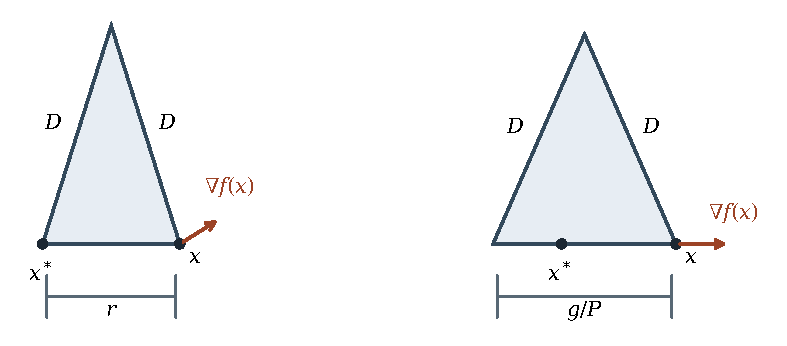
\includegraphics[width=0.9\linewidth]{figures/diameter_geometry.pdf}
\caption{Sharpness constructions for feasible exact observations. Left: gap-active data, $g\le P^2/m$. Right: norm-active data, $P^2/m<g\le PD$. Both sloping sides have length $D$.}
\label{jointdiam:geometry}
\end{figure}

\paragraph{Proof of Theorem~\ref{jointdiam:main}.}
The definitions give $0<\rho_-\le\rho_+$; continuity of $V$ ensures
that the maximum exists. For a nonoptimal source,
write $r=\|x-x^*\|$ and let $p$ be its terminal radial derivative.
Shifted RSI and constrained minimality give
$mr\le p\le P$, while $pr\le G(x)\le g$ and $r\le D$. Hence
\[
 pr\le\min\{g,P^2/m,PD\}=h,\qquad
 r\le R:=\min\{\sqrt{h/m},D\}.
\]
Put $r_0=h/P\le R$. The radial envelope $A(P,r)$ in
\eqref{joint:radial-identity} is strictly increasing in $r$.
For $r\le r_0$ it bounds the loss by
$A(P,r_0)=V(h,r_0^2)$. For $r\ge r_0$, the terminal cap $h/r$
and initial cap $h/r-mr$ bound it by $V(h,r^2)$. This proves
\eqref{jointdiam:definition}. A zero gap or zero norm forces zero
error by shifted RSI. The zero bound is attained at the minimizer
of a quadratic on a triangle of diameter $D$.

For sharpness, choose a maximizing radius $\rho$, and put
\[
 r=\sqrt\rho,\quad p=h/r,\quad q=p-mr,\quad
 c=\sqrt{P^2-p^2},\quad a_D=\sqrt{D^2-r^2/4}.
\]
The scalar construction in Lemma~\ref{compact:radial} gives
smooth functions $u_j$ on neighborhoods of $[0,r]$ with
\[
 \begin{gathered}
 u_j(0)=0,\quad u_j'(0)=q,\quad u_j'(r)=p,\quad
 u_j'(s)-q\ge ms,\\
 |u_j''(s)|\le H_0+H_1u_j(s),\qquad
 u_j(r)\longrightarrow V(h,\rho).
 \end{gathered}
\]
Define
\[
 Q=\operatorname{conv}\{(0,0),(r,0),(r/2,a_D)\},\qquad
 f_j(s,y)=u_j(s)+cy+my^2/2.
\]
The two sloping sides have length $D$ and the base has length
$r\le D$, so $Q$ has diameter exactly $D$ and nonempty interior.
Its points satisfy $0\le s\le r$ and $y\ge0$. The unique minimizer
is $(0,0)$, and throughout $Q$,
\[
 \langle\nabla f_j(s,y)-\nabla f_j(0,0),(s,y)\rangle
       =(u_j'(s)-q)s+my^2\ge m(s^2+y^2),
\]
\[
 \|\nabla^2f_j(s,y)\|
       =\max\{|u_j''(s)|,m\}
       \le H_0+H_1u_j(s)\le H_0+H_1f_j(s,y).
\]
At $(r,0)$ the gradient is $(p,c)$, of norm $P$. Its linear
pairing is minimized at $(0,0)$, so the full gap is $pr=h\le g$.
The source loss tends to $\mathcal J_D(g,P)$. This proves sharpness
for upper bounds, even with diameter fixed exactly.

For exact positive observations, $g\le PD$ is necessary by
$G(x)\le\|\nabla f(x)\|\operatorname{diam}Q$. If also
$g\le P^2/m$, then $h=g$, and the preceding construction already
has both observations exact. If $P^2/m<g\le PD$, set
\[
 r=P/m,\qquad a=g/P-r,\qquad \ell=r+a=g/P\le D.
\]
Use smooth scalar profiles on $[0,r]$ with initial slope zero
and terminal slope $P$, approaching $\mathcal E(P)$. Their
smoothing is confined to the interior switch, so near zero
they agree with
\[
 u_+(s)=
 \begin{cases}
 (H_0/H_1)\{\cosh(\sqrt{H_1}s)-1\},&H_1>0,\\
 H_0s^2/2,&H_1=0.
 \end{cases}
\]
Extend them to $[-a,0]$ by this even function. There
$|u_+''|=H_0+H_1u_+$ and $u_+'(s)s\ge ms^2$.
Denote the extension by $u_j$.
On the triangle
\[
 Q=\operatorname{conv}\left\{(-a,0),(r,0),
       \left((r-a)/2,\sqrt{D^2-\ell^2/4}\right)\right\}
\]
put $f_j(s,y)=u_j(s)+my^2/2$. Again $\operatorname{diam}Q=D$,
the minimizer is $(0,0)$, and shifted RSI and the Hessian bound
hold on all of $Q$. The source gradient is $(P,0)$; the linear
oracle selects $(-a,0)$, giving gap $P\ell=g$. The loss tends
to $\mathcal E(P)=\mathcal J_D(g,P)$. All the functions are
smooth on neighborhoods of their triangles.

Formula \eqref{jointdiam:constant} maximizes the affine radius
profile $h+\beta\rho$. Formula \eqref{jointdiam:ordinary} follows
from Corollary~\ref{gapregime:radius-monotone} at $\rho_-$.
For Corollary~\ref{jointdiam:norm}, the gap bound $PD$ follows
from the norm and diameter bounds. In
$\mathcal J_D(PD,P)$ the radius interval is the singleton
$r_D^2$, and its initial slope is
$P-mr_D=\max\{P-mD,0\}=q$. The radial identity and
Proposition~\ref{joint:fixed-slope} give
\eqref{jointdiam:norm-formula}; the constant-curvature radius
formula gives \eqref{jointdiam:norm-constant}.

\paragraph{The full gap with a known diameter.}
For $D>0$ define
\begin{equation}\label{compact:gap-diameter}
 \mathcal B_D(g)=
 \max_{0\le\rho\le\min\{g/m,D^2\}}V(g,\rho),\qquad
 \mathcal B_D(0)=0.
\end{equation}
If $\operatorname{diam}Q\le D$, then
$\delta(x)\le\mathcal B_D(G(x))\le\mathcal B(G(x))$.
This is the exact supremum for a fixed full gap and a diameter
bound. The function $\mathcal B_D$ is continuous and satisfies
\eqref{boundarygap:growth}.

Indeed, the radial upper bound uses $r\le D$, and the smooth
examples on $[0,r]$ from Lemma~\ref{compact:radial} approach
every value with $r\le D$. The same quadratic functions plus
a linear term as in the proof of Theorem~\ref{boundarygap:main}
give the limit $\rho\downarrow0$.
The substitution $\rho=z\min\{g/m,D^2\}$, $z\in[0,1]$, proves
continuity; adding a linear term proves growth without changing
the interval length.

For $H_1=0$,
\[
 \mathcal B_D(g)=g+\max\{0,\beta\}\min\{g/m,D^2\}.
\]
For $H_1>0$, $g>0$, the exact criterion is
\[
 \mathcal B_D(g)=g\quad\Longleftrightarrow\quad\mathcal S(g)\le0.
\]
In the nonpositive case, use
$g\le\mathcal B_D(g)\le\mathcal B(g)=g$.
In the positive case, the first variation
\eqref{gapregime:variation} exceeds $g$ at arbitrarily small
positive radii, which also satisfy $\rho\le D^2$.
For scalar evaluation, apply Proposition~\ref{boundarygap:budget}
on the shorter interval with $\ell=g$.

\section{Adaptive stopping and complete query counts}
\label{nloracle:section}
The certificates above can be used with ordinary quadratic backtracking.
We state the work bound once for a general calibration $\Phi$; the
specializations then change only this function. Objective values are exact.
Let $D\ge\operatorname{diam}Q>0$, and suppose
\begin{equation}\label{nloracle:model}
 \lambda_{\max}(\nabla^2f(x))\le K(\delta(x)),\qquad
 \delta(x)\le\Phi(G(x)).
\end{equation}
Here $K:[0,\infty)\to[0,\infty)$ is finite, continuous and nondecreasing,
and $\Phi:[0,\infty)\to[0,\infty)$ is continuous,
strictly increasing and unbounded, with $\Phi(0)=0$.
The sharp gap envelope gives $\Phi=\mathcal B$ and $K(u)=H_0+H_1u$.
The known diameter also permits $\Phi=\mathcal B_D$.
These stopping assumptions also allow other regularity conditions.

At requested directional accuracy $\eta>0$, a query returns $h\ge0$
and $d=s-x$, $s\in Q$, such that
\begin{equation}\label{nloracle:query}
 G(x)\le B=h+\eta,\qquad
 -\langle\nabla f(x),d\rangle\ge h-\eta.
\end{equation}
A source certificate $C$ must satisfy $\delta(x)\le C\le\Phi(B)$.
One may use $C=\Phi(B)$ or a sharper valid joint certificate.
Retain $\ell\leftarrow\max\{\ell,f(x)-C\}$ and set $U=f(x)-\ell$.
The initial query creates the first lower bound.

\paragraph{The rule.}
Choose $\eta_0,M>0$ and $0<\theta<1$, and carry $\eta$ between points.
After every query, first stop if $U\le\varepsilon$, where $\varepsilon>0$.
Otherwise require $\eta\le\theta h$. If this fails, halve $\eta$ and
query at the same point, reusing its objective value.
After it passes, put $a=h-\eta$, start with $L=L_{k-1}/2$,
$L_{-1}=M$, and double $L$ until
\begin{equation}\label{eq:btstep}
 \alpha=\min\{1,a/(L\|d\|^2)\},\qquad
 f(x+\alpha d)\le f(x)-\alpha a+\tfrac12L\alpha^2\|d\|^2.
\end{equation}
Accept $x+\alpha d$, cache its value, and retain the accepted $L_k$.
This is the usual backtracking update \cite{pedregosa}; the new
certificates determine when its computed points are accurate enough.

\begin{theorem}[Stopping with carried accuracy]\label{nloracle:main}
Every refinement loop and line search terminates, and the rule stops
with $\delta(x_N)\le U_N\le\varepsilon$.
Let $N$ count accepted updates and $R$ count accuracy halvings, including
initial and terminal source checks. With $\kappa=(1-\theta)/(1+\theta)$,
\begin{equation}\label{nloracle:refinement}
 R\le\left\lceil\log_2\max\left\{1,
 \frac{(1+\theta)\eta_0}{\theta\Phi^{-1}(\varepsilon)}\right\}\right\rceil,
 \qquad T=N+1+R.
\end{equation}
There are exactly $T$ source queries. Each vector query followed by a
full LMO costs one LMO; each score query below costs one full atom scan.

If an initial update is needed, let $U_0>\varepsilon$ be the certificate
after its precision check, and set
\[
 \begin{gathered}
 J=\lceil\log_2(U_0/\varepsilon)\rceil,\quad b_j=U_0/2^j,\quad
 s_j=\kappa\Phi^{-1}(b_j/2),\\
 C_j=\max\{2K(b_j),s_j/D^2\},\quad
 P_K=\left\lceil\log_2\frac{\max\{M,C_0\}}{C_{J-1}}\right\rceil,
 \qquad 0\le j<J.
 \end{gathered}
\]
Then
\begin{equation}\label{nloracle:work}
 N\le T_\varepsilon:=P_K+
 \left\lceil\sum_{j=0}^{J-1}
 \max\left\{\frac{2b_j}{s_j},\frac{4D^2K(b_j)b_j}{s_j^2}\right\}\right\rceil.
\end{equation}
For actual $N\ge1$, all line-search objective calls, including the
initial value and rejected trials, satisfy
\begin{equation}\label{nloracle:functions}
 N_f\le1+2N+
 \left\lceil\log_2\max\{1,2K(U_0)/M\}\right\rceil.
\end{equation}
If $N=0$, there is one objective call and $1+R$ source queries.
The phase quantities are then unnecessary.
\end{theorem}

\begin{proof}
Every retained lower bound is valid, so $0\le\delta\le U\le C\le\Phi(B)$.
At a nonterminal failed precision check,
\[
 \Phi^{-1}(\varepsilon)<\Phi^{-1}(U)\le B
   <(1+\theta)\eta/\theta.
\]
Since the precision is halved and never reset, this proves the bound on
$R$ and finiteness of each check. Each visited point has one closing
query, and each halving has one additional failed query. Hence $T=N+1+R$.
At a passed nonterminal check,
\begin{equation}\label{compact:certified-slope}
 a=h-\eta\ge\kappa(h+\eta)\ge\kappa\Phi^{-1}(U)>0.
\end{equation}

For the line search put $w(t)=f(x+td)-f(x)$ and $K_x=K(\delta(x))$.
While $w\le0$, $w''\le K_x\|d\|^2$ and $w'(0)\le-a<0$.
A first return to zero before $2a/(K_x\|d\|^2)$ contradicts
$w(t)\le-at+K_x\|d\|^2t^2/2<0$. Thus every $L\ge K_x$
passes the test at its proposed step. If $K_x=0$, use the linear
comparison. Every accepted trial satisfies
\begin{equation}\label{eq:acceptedprogress}
 f_k-f_{k+1}\ge\alpha_k a_k/2,\qquad
 L_k\le\max\{L_{k-1}/2,2K(\delta_k)\}.
\end{equation}
The objective decreases and the retained lower bound increases, so $U$
is nonincreasing, also during refinements at a fixed point.

Assign a nonterminal update to $b_j/2<U_k\le b_j$.
The positive phase caps $C_j$ are nonincreasing. If $L_k>C_j$,
the accepted trial must have been the first one: otherwise the preceding
rejected value would be at least $C_j/2\ge K(\delta_k)$.
Such an update therefore halves the inherited curvature.
Before an update in phase $j$, use
\[
 V_k=\max\{0,\log_2(L_{k-1}/C_j)\}.
\]
An update above the cap reduces this potential by one; an update below
the cap leaves zero before a phase change. A jump from phase $j$ to
$j'$ increases it by at most $\log_2(C_j/C_{j'})$. These increments
telescope, so there are at most $P_K$ updates above their caps.

At any remaining update, \eqref{compact:certified-slope} and $\|d\|\le D$
give objective decrease at least
\[
 p_j=\min\{s_j/2,s_j^2/(2C_jD^2)\}=s_j^2/(2C_jD^2).
\]
The total decrease from points in phase $j$ is at most the true error
at its entry, hence at most $b_j$. There are at most $b_j/p_j$ such
updates. Summation proves \eqref{nloracle:work}. The same finite bound
holds for every unfinished prefix, excluding an infinite nonterminal run.

If $q_k$ trials are rejected at update $k$, then
$L_k=2^{q_k-1}L_{k-1}$. Consequently
\[
 \sum_{k<N}(q_k+1)=2N+\log_2(L_{N-1}/M),\qquad
 L_{N-1}\le\max\{M/2^N,2K(U_0)\}.
\]
Adding the initial objective call proves \eqref{nloracle:functions}.
\end{proof}

\paragraph{Away steps.}\label{alg:afw}
For $Q=\operatorname{conv}\mathcal A$ with finitely many atoms, maintain
exact positive weights on the active set $S$.
For AFW, the full LMO returns a minimizing atom in $\mathcal A$, including ties.
Use $B=h_{\rm FW}+\eta$ for stopping and the FW precision check.
Only after that check passes,
scan the active set and compare its approximate away gap with the FW gap.
Select the larger, use FW on ties and singleton sets,
and subtract $\eta$ from the selected gap. The error guarantee must
hold uniformly for both directions, as in the next section.
The away direction $x-v$ has cap $\lambda_v/(1-\lambda_v)$; replace
the cap $1$ in \eqref{eq:btstep} by this value \cite{lacostejaggi}.
A step that reaches the away cap removes an atom. Every other step has
the same progress bound as a FW step. The potential proof counts all
updates above their caps, and the decrease proof counts the remaining
good updates. Thus good updates number at most $T_\varepsilon$.
FW adds at most one atom and a drop removes one, giving
\begin{equation}\label{eq:dropcount}
 N\le2T_\varepsilon+|S_0|-1.
\end{equation}
The query and objective bounds use this actual total $N$; AFW also
performs $N$ active-set scans.

\begin{corollary}[Certified scalar evaluation]\label{nloracle:energy}
Suppose $\delta\le\Phi_0(G)$ and a scalar routine returns
$\Phi_0(B)\le\widehat\Phi_0(B)\le\vartheta\Phi_0(B)$ for known
$\vartheta\ge1$. Use $C=\widehat\Phi_0(B)$, or the smaller of this
value and any other valid source bound. The theorem applies with
$\Phi=\vartheta\Phi_0$. In particular, one may take
$\Phi_0=\mathcal B$ or $\Phi_0=\mathcal B_D$; under $\nabla f(x^*)=0$, one may also take
$\Phi_0=W$. The inverse is needed in the analysis, not in the algorithm.
\end{corollary}
\begin{proof}
Validity gives $\delta\le C$, and construction gives
$U\le C\le\vartheta\Phi_0(B)$. These are the calibration inequalities
used in the proof. The required properties of $\mathcal B$ and $W$
were proved above.
\end{proof}

A norm enclosure $P^+$ permits the exact choice $C=\mathcal J_D(B,P^+)$.
For a computed enclosure, use
$C=\widehat{\mathcal J}_D(B,P^+)\le\vartheta\mathcal J_D(B,P^+)
\le\vartheta\mathcal B_D(B)$ and the effective calibration
$\Phi=\vartheta\mathcal B_D$. The last inequality follows from the
cap characterization of $\mathcal J_D$. Either choice can be combined with other
valid source bounds by taking their minimum. Norm formation and scalar
evaluation are additional work.
If the scalar routine uses $n(B_j)$ comparisons at query $j$, charge
$\sum_{j=1}^{N+1+R}n(B_j)$, including failed refinements and the terminal
query. Comparison counts alone do not bound interval or bit arithmetic.
For a nonincreasing query-cost bound $C_{\rm query}(\eta)$, the total is
at most
\[
 (N+1)C_{\rm query}(\eta_R)+\sum_{r=0}^{R-1}C_{\rm query}(\eta_0 2^{-r}).
\]

\paragraph{Linear gap bounds and the final phases.}
A known $G\ge\gamma\delta$ with $\gamma>0$ gives $\Phi(g)=g/\gamma$.
For $K(u)=H_0+H_1u$ and $\bar\gamma=\kappa\gamma$,
\eqref{nloracle:work} implies
\[
 N\le P_K+\left\lceil
 \frac{4J}{\bar\gamma}+
 \frac{32D^2H_0}{\bar\gamma^2\varepsilon}+
 \frac{16D^2H_1J}{\bar\gamma^2}\right\rceil.
\]
Indeed $s_j=\bar\gamma b_j/2$ and
$\sum_{j<J}b_j^{-1}<2/\varepsilon$.
Quasar-convexity with center $x^*$ supplies this gap bound through
$\langle\nabla f(x),x-x^*\rangle\ge\gamma\delta(x)$.
It need not imply convexity between arbitrary pairs of points.
For the sharp shifted-RSI calibration, the phases with
$b_j/2\le g_c$ have $\mathcal B^{-1}(b_j/2)=b_j/2$ whenever the
positive threshold $g_c$ exists. Their progress bound therefore has
the same form with $\gamma=1$.
For $\Phi=\vartheta\mathcal B$, the corresponding condition is
$b_j/(2\vartheta)\le g_c$, and $s_j=\kappa b_j/(2\vartheta)$.
The same final-phase formulas hold for $\mathcal B_D$, whose ordinary-gap
regime is identical.

\section{Directional errors and finite-variance observations}
\label{diroracle:section}
We give two implementations of \eqref{nloracle:query} and one sampling
construction. Median-of-means estimation is classical \cite{dirlugosi};
robust stochastic FW is studied in \cite{dirtang,dirsfyraki}.
Here it supplies the stated global-error stopping certificate with
exact objective values.

\begin{proposition}[Vector and score implementations]
\label{diroracle:width-transfer}\label{diroracle:scores}
Define the feasible-direction seminorm
\[
 \omega_Q(v)=\max_{u,w\in Q}\langle v,u-w\rangle\le D\|v\|.
\]
If a vector query satisfies $\omega_Q(\widehat g-\nabla f(x))\le\eta$,
choose $s\in\arg\min_{v\in Q}\langle\widehat g,v\rangle$ and
$h=\langle\widehat g,x-s\rangle$. Then \eqref{nloracle:query} holds,
also for the selected away direction with its own approximate gap.

Alternatively let $Q=\operatorname{conv}\{v_0,\ldots,v_{n_A-1}\}$,
$n_A\ge2$, and $x=\sum_i\lambda_i v_i$ with exact nonnegative weights
summing to one. Put $t_i=\langle\nabla f(x),v_i-v_0\rangle$.
Suppose $q_0=t_0=0$ and
\begin{equation}\label{diroracle:score-error}
 \max_i(q_i-t_i)-\min_i(q_i-t_i)\le\eta.
\end{equation}
Set $q_x=\sum_i\lambda_iq_i$, choose $i_s\in\arg\min_i q_i$, and
use $h=q_x-q_{i_s}$. This also gives \eqref{nloracle:query} and the
away-direction guarantee. The scores need not be a linear functional.
Each query then costs a full scan of $n_A$ scores.
\end{proposition}
\begin{proof}
The seminorm bounds the absolute error on each difference of feasible
points by $\eta$. Taking the maximum proves the gap bound; evaluating
the selected direction proves the slope bound.
For scores write $e_i=q_i-t_i$ and $e_x=\sum_i\lambda_i e_i$.
The error $e_x$ lies between the smallest and largest $e_i$, so
\[
 \langle\nabla f(x),x-v_i\rangle=q_x-q_i-e_x+e_i\le h+\eta.
\]
The selected FW slope is at least $h-\eta$. The away slope is at least
$q_i-q_x-\eta$. Also $h\ge0$ because $q_x$ is a convex combination.
\end{proof}

For a Euclidean error bound $\eta_{\rm norm}$, use
$\eta=D\eta_{\rm norm}$ and $P^+=\|\widehat g\|+\eta_{\rm norm}$.
The latter can feed the joint certificate. Directional or score errors
alone do not imply such a norm bound. On the radius-$R$ $\ell_1$ ball,
$\omega_Q(v)=2R\|v\|_\infty$; on the simplex it is
$\max_i v_i-\min_i v_i$. Enumerating scores is not one black-box LMO
call on an implicit polytope.

At a requested point suppose one fresh observation gives $n_A-1$
scalar values $Y_i$. Conditional on the entire past $\mathcal F$,
observations within the query are independent and identically distributed,
with known uniform bound
\begin{equation}\label{diroracle:moment}
 \mathbb E[Y_i\mid\mathcal F]=t_i(x),\qquad
 \mathbb E[(Y_i-t_i(x))^2\mid\mathcal F]\le\sigma_A^2<\infty.
\end{equation}
Coordinates of one observation may be dependent.
Number every query, including refinements, by $j\ge1$.
At precision level $r$, let $\eta_r=\eta_0 2^{-r}$ and choose
\begin{equation}\label{diroracle:batch}
 b_r=\max\{1,\lceil16\sigma_A^2/\eta_r^2\rceil\},\qquad
 k_j=2\left\lceil4\log\frac{(n_A-1)j(j+1)}\zeta\right\rceil+1,
 \quad 0<\zeta<1.
\end{equation}
Draw $b_rk_j$ observations. For each coordinate, take the median of
the $k_j$ means over disjoint blocks of size $b_r$; set $q_0=0$.

\begin{theorem}[One confidence event for all queries]\label{diroracle:sampling}
With probability at least $1-\zeta$, every query requested by the
algorithm satisfies \eqref{diroracle:score-error}. On this event all
bounds of Theorem~\ref{nloracle:main} hold, including
$\delta(x_N)\le U_N\le\varepsilon$ at its random stopping time.
For actual $T=N+1+R$, the number of raw observations satisfies
\begin{align}\label{diroracle:samples}
 S&\le k_T\left[(N+1)b_R+\sum_{r=0}^{R-1}b_r\right]\\
  &\le k_T\left[T+16\sigma_A^2\eta_R^{-2}
       \left(N+1+\frac{1-4^{-R}}3\right)\right].\nonumber
\end{align}
Each observation returns all $n_A-1$ coordinates, so it represents
$(n_A-1)S$ scalar directional values. Medians, scans and exact
objective evaluations are separate costs.
\end{theorem}
\begin{proof}
Conditional Chebyshev gives a probability at most $1/4$ that one block
mean has error greater than $\eta_r/2$. For $\sigma_A=0$ this probability
is zero. Independence of the blocks and Hoeffding's bound show that
the odd median fails only with probability at most $e^{-k_j/8}$.
A union bound over coordinates gives conditional failure probability
at most $\zeta/[j(j+1)]$. Coordinate errors at most $\eta_r/2$
give a score-error range at most $\eta_r$.
Apply this bound on the event that query $j$
is requested, take expectations, and sum over all $j\ge1$.
Since the sum of $1/[j(j+1)]$ is one, all queries are valid together
with probability at least $1-\zeta$. The deterministic prefix proof
then establishes termination without a fixed query horizon.

There is one failed query at each level $0,\ldots,R-1$ and $N+1$
closing queries at levels at most $R$. Since $k_j$ increases, this
gives the first sample bound. The second uses
$b_r\le1+16\sigma_A^2\eta_r^{-2}$ and
$\sum_{r<R}\eta_r^{-2}=\eta_R^{-2}(1-4^{-R})/3$.
\end{proof}

The directional moment assumption can hold without an ambient vector
moment. On a simplex, a common Cauchy component $W\mathbf1$ cancels
from every difference $\langle Z,e_i-e_0\rangle$. The differences
must still have the finite conditional variance in
\eqref{diroracle:moment}. The construction requires a finite explicit
atom set, fresh samples, a known variance bound and exact objectives.

\section{Application to realizable sigmoid regression}
\label{reg:sigmoid}
Realizable generalized linear models have known quasar-convexity
guarantees \cite[Lemma 3]{regglm}; derivative-ratio alignment is also
used in \cite[Lemma 5]{regfoster}. Sigmoid least squares on an
$\ell_1$ ball is an existing conditional-gradient benchmark
\cite[Section 5.1.4]{khademi}. We give explicit constants for the
certificates above.

Let $A\in\mathbb R^{n\times d}$ have rows $a_i^\top$, let
$Q=\{x:\|x\|_1\le R\}$, $R>0$, and fix $x^*\in Q$.
For $\sigma(z)=(1+e^{-z})^{-1}$ and targets
$y_i=\sigma(a_i^\top x^*)$, define
\begin{equation}\label{reg:sigmoidloss}
 f(x)=\frac1{2n}\sum_{i=1}^n[\sigma(a_i^\top x)-y_i]^2.
\end{equation}
Then $f^*=0$ and $\nabla f(x^*)=0$. Set
\[
 \begin{gathered}
 Z=R\max_i\|a_i\|_\infty,\qquad
 m_\sigma=(2+2\cosh Z)^{-1},\quad
 M_\sigma=1/4,\quad C_\sigma=1/(6\sqrt3),\\
 S=A^\top A/n,\quad \lambda=\lambda_{\min}(S),\quad
 \Lambda=\lambda_{\max}(S),\quad K_A=\max_i\|a_i\|^2.
 \end{gathered}
\]
Every feasible score lies in $[-Z,Z]$, where
$m_\sigma\le\sigma'\le M_\sigma$; globally $|\sigma''|\le C_\sigma$.

\begin{proposition}[Regularity and curvature constants]
\label{reg:sigmoidbounds}
If $\lambda>0$, the objective satisfies shifted RSI with
$m=m_\sigma^2\lambda$. For every $t>0$ it satisfies the Hessian-norm
bound with
\begin{equation}\label{reg:sighess}
 H_0=\Lambda\left(M_\sigma^2+\frac{C_\sigma^2}{2t}\right),
 \qquad H_1=K_A t.
\end{equation}
It also satisfies
\begin{equation}\label{reg:quasar}
 \langle\nabla f(x),x-x^*\rangle\ge\gamma f(x),\qquad
 \gamma=\min\{1,2m_\sigma/M_\sigma\}>0,
\end{equation}
and has the global feasible-region bound
\begin{equation}\label{reg:sigglobal}
 \|\nabla^2f(x)\|\le L_Q
 :=\Lambda\bigl(M_\sigma^2+C_\sigma\tanh(Z/2)\bigr).
\end{equation}
The last two conclusions hold without full column rank.
\end{proposition}
\begin{proof}
Write $d=x-x^*$, $z_i=a_i^\top x$ and
$r_i=\sigma(z_i)-\sigma(a_i^\top x^*)$.
The mean-value theorem gives $r_i=\bar s_i a_i^\top d$ with
$\bar s_i\in[m_\sigma,M_\sigma]$. Hence
\[
 \langle\nabla f(x),d\rangle
 =\frac1n\sum_i\bar s_i\sigma'(z_i)(a_i^\top d)^2
 \ge m_\sigma^2d^\top Sd\ge m\|d\|^2.
\]
The same sum equals
$n^{-1}\sum_i\sigma'(z_i)r_i^2/\bar s_i
 \ge 2m_\sigma f(x)/M_\sigma$, proving \eqref{reg:quasar}.
The Hessian is
\[
 \nabla^2f(x)=\frac1n\sum_i
 [\sigma'(z_i)^2+r_i\sigma''(z_i)]a_i a_i^\top.
\]
For a unit vector $v$, Cauchy-Schwarz and
$(a_i^\top v)^4\le K_A(a_i^\top v)^2$ bound its absolute quadratic
form by
\[
 M_\sigma^2\Lambda+C_\sigma\sqrt{2K_A\Lambda f(x)}
 \le\Lambda\left(M_\sigma^2+\frac{C_\sigma^2}{2t}\right)+K_Atf(x).
\]
This proves \eqref{reg:sighess}. Using
$|r_i|\le\tanh(Z/2)$ instead gives \eqref{reg:sigglobal}.
\end{proof}

The application includes nonconvex objectives. Take $n=d=1$,
$Q=[-2,2]$, $a_1=1$ and $x^*=-2$. For
$q=\tanh1>1/2$ and $p=\sigma'(2)=(1-q^2)/4$,
\[
 f''(2)=p^2-pq^2=\frac p4(1-5q^2)<0.
\]
Continuity gives negative curvature at nearby interior points as well.

The constants require exact realizability. Arbitrary noisy targets
do not inherit these zero-floor RSI and alignment guarantees.
Large $Z$ can also make $m_\sigma$ very small, so the bounds may be
conservative. Both the affine curvature model and $L_Q$ are valid;
neither is uniformly the better description. The parameter $t$ selects
a bound and is not a line-search parameter.

The diameter of the $\ell_1$ ball is $D=2R$. Thus full column rank
allows all norm, gap and joint certificates, including $\mathcal J_D$;
\eqref{reg:quasar} alone allows the linear-gap stopping bound.
If the solver is told that the targets are realizable by a feasible
point, it already knows $f^*=0$, so $f(x)$ itself certifies the error.
A comparison that withholds this lower bound must state that choice.
The constrained model does not assert an equivalence with a fixed
$\ell_1$ penalty for arbitrary nonconvex objectives.

\section{Certificate evaluation and computational evidence}
\label{compact:evidence}
The proofs establish the envelopes; the computations below check
their formulas and implementation. They do not search for theorems
or infer global maxima from sampled radii. The accompanying code
uses exact rational inputs, outward interval arithmetic, explicit
resource limits and structured refusals when it cannot certify a result.

\begin{table}[htbp]
\centering
\caption{Fixed certificate comparisons. The first and third rows are
exact. The second row abbreviates a certified interval.}
\label{compact:certificate-table}
\begin{tabular}{lccc}
\toprule
$(m,H_0,H_1;g,P)$ & Separate bounds & $\mathcal J(g,P)$ & $\mathcal J_D(g,P)$\\
\midrule
$(1,1,0;1/2,1)$ & $1/2$ & $3/8$ & not used\\
$(1,1,1;1,2)$ & $1$ & $0.903217\ldots$ & not used\\
$(1,4,0;1,2)$ & $23/16$ & $23/16$ & $463/400$ for $D=3/5$\\
\bottomrule
\end{tabular}
\end{table}
Here ``separate bounds'' means
$\min\{\mathcal B(g),\mathcal E(P)\}$.
In the second row, the frozen scalar calculation gives
\[
 \begin{aligned}
 0.90321723720789&<\mathcal J(1,2)<0.90321723720790,\\
 2.56989673908727&<\mathcal E(2)<2.56989673908729.
 \end{aligned}
\]
The gap envelope equals one. The algebraic upper bound
$2-7\sqrt{14}/24=0.908683\ldots$ also improves it.
Radius monotonicity proves that the selected endpoint is the joint
maximum. The calculation uses 100 decimal digits and 96 switch
bisections per fixed radius; the saved record includes independent
travel-time enclosures. The diameter example satisfies $g<PD$, so
the improvement persists when both observations are exact.

The retained v16 API panel has 16 prescribed calls, 12 certified
outputs and four expected refusals, with 238 assertions in its control
script. The earlier v15 panel is a separate record with 26 calls and
503 assertions. Neither count is a number of optimization experiments.
The diameter extension has a separate first run of ten prescribed
calls: seven certified outputs, three expected refusals and 184 control
assertions. It used 113 named scalar evaluations and 61 bisection
updates. The release evidence file gives the individual outcomes and
separate operation counts. The API rejects
binary floating-point inputs rather than silently treating rounded
observations as exact. A refusal does not invalidate the analytic bound.

The earlier optimization records are retained in a separate archive.
For example, the fixed empirical monitor certified five of 16 saved
paths; a separate study on six selected endpoints certified three.
These sets have different selection rules and are not pooled.
They concern the previous application monitors, not a runtime test of
$\mathcal J_D$. This revision adds no optimizer trajectories, LP solves
or stochastic samples. Formula checks and manuscript verification are
recorded separately from the costs of an optimization algorithm.

\section{Scope and further questions}
The sharp bounds use known regularity and curvature constants.
Estimating those constants from a finite sample of derivatives does
not verify the assumptions on the whole feasible set. The sigmoid
application supplies analytic constants under its stated model;
other applications need their own justification.

Diameter information improves the best bound over varying domains.
A fixed polytope, a known active face or additional derivative data can
carry more information than $(g,P,D)$. Determining the corresponding
sharp certificates is a separate problem. The possible nonconcavity
of the radius profile also leaves room for certified maximization
schemes more efficient than the general finite grid.

The stopping theorem assumes exact objective values. Its stochastic
implementation additionally requires fresh directional observations,
a finite explicit atom set and a known variance bound. No guarantee
for noisy objectives or unknown variances follows without further
analysis. The scalar comparison budgets do not give bit complexity
or a runtime bound for interval arithmetic.

\paragraph{Reproducibility.}
The public release contains both manuscript sources, scalar certificate
code, frozen scalar protocols and first-run results. Extended earlier
proofs and optimization records are retained in a separate archive.

\paragraph{AI assistance.}
AI tools assisted with mathematical drafting, code, translation and
editing. The recorded checks are numerical or analytic reviews, not
formal proof verification.

\begin{thebibliography}{99}
\bibitem{warmup}F.~Alimisis, R.~Islamov, and A.~Lucchi.
Why Do We Need Warm-up? A Theoretical Perspective.
\href{https://arxiv.org/abs/2510.03164v2}{arXiv:2510.03164v2}, 2026.

\bibitem{vyguzov}A.~A.~Vyguzov, F.~S.~Stonyakin, and A.~V.~Gasnikov.
Frank-Wolfe Algorithms for $(L_0,L_1)$-smooth functions.
\emph{Journal of Nonlinear and Variational Analysis}, 10(3):597-616, 2026.
\href{https://doi.org/10.23952/jnva.10.2026.3.05}{doi:10.23952/jnva.10.2026.3.05}.

\bibitem{regregularity}Y.~Zhou and Y.~Liang.
Characterization of Gradient Dominance and Regularity Conditions for Neural Networks.
\href{https://arxiv.org/abs/1710.06910v2}{arXiv:1710.06910v2}, 2017.

\bibitem{rsipep}C.~Guille-Escuret, A.~Ibrahim, B.~Goujaud,
and I.~Mitliagkas.
Gradient Descent Is Optimal Under Lower Restricted Secant Inequality
And Upper Error Bound.
\emph{Advances in Neural Information Processing Systems}, 35, 2022.
\href{https://proceedings.neurips.cc/paper_files/paper/2022/file/9daab3b451038ed1bc5d8e9b77996b99-Paper-Conference.pdf}{NeurIPS proceedings}.

\bibitem{pedregosa}F.~Pedregosa, G.~Negiar, A.~Askari, and M.~Jaggi.
Linearly Convergent Frank-Wolfe with Backtracking Line-Search.
\emph{AISTATS}, 2020. \href{https://arxiv.org/abs/1806.05123}{arXiv:1806.05123}.

\bibitem{lacostejaggi}S.~Lacoste-Julien and M.~Jaggi.
On the Global Linear Convergence of Frank-Wolfe Optimization Variants.
\emph{NeurIPS}, 2015.
\href{https://arxiv.org/abs/1511.05932}{arXiv:1511.05932}.

\bibitem{oraclehallak}N.~Hallak and K.~Y.~Levy.
A Study of First-Order Methods with a Deterministic Relative-Error Gradient Oracle.
\emph{Proceedings of the 41st International Conference on Machine Learning},
PMLR 235:17313-17332, 2024.
\url{https://proceedings.mlr.press/v235/hallak24a.html}.

\bibitem{oracledenisov}G. Denisov, F. Stonyakin, and M. Alkousa.
Adaptive Variants of Frank-Wolfe Method with Relative Inexact
Gradient Information.
\emph{Mathematical Optimization Theory and Operations Research},
LNCS 15681, pp. 3 to 16, 2025.
\url{https://doi.org/10.1007/978-3-031-97077-1_1}.

\bibitem{dirlugosi}G. Lugosi and S. Mendelson.
Mean estimation and regression under heavy-tailed distributions: a survey.
\emph{Foundations of Computational Mathematics}, 19:1145-1190, 2019.
\href{https://arxiv.org/abs/1906.04280}{arXiv:1906.04280}.

\bibitem{dirtang}T. Tang, K. Balasubramanian, and T. C. M. Lee.
High-probability bounds for robust stochastic Frank-Wolfe algorithm.
\emph{Proceedings of the Thirty-Eighth Conference on Uncertainty in
Artificial Intelligence}, PMLR 180:1917-1927, 2022.
\href{https://proceedings.mlr.press/v180/tang22a.html}{Publisher page}.

\bibitem{dirsfyraki}M.-E. Sfyraki and J.-K. Wang.
Lions and Muons: Optimization via stochastic Frank-Wolfe under
heavy-tailed noise.
\emph{Proceedings of the 43rd International Conference on Machine
Learning}, PMLR 306:109388-109428, 2026.
\href{https://proceedings.mlr.press/v306/sfyraki26a.html}{Publisher page}.

\bibitem{regglm}J.-K.~Wang and A.~Wibisono.
Continuized Acceleration for Quasar Convex Functions in Non-Convex Optimization.
\emph{ICLR}, 2023.
\href{https://arxiv.org/abs/2302.07851}{arXiv:2302.07851}.

\bibitem{regfoster}D.~J.~Foster, A.~Sekhari, and K.~Sridharan.
Uniform Convergence of Gradients for Non-Convex Learning and Optimization.
\emph{Advances in Neural Information Processing Systems}, 31, 2018.
\href{https://arxiv.org/abs/1810.11059v2}{arXiv:1810.11059v2}.

\bibitem{khademi}A.~Khademi and A.~Silveti-Falls.
Adaptive Conditional Gradient Descent.
\href{https://arxiv.org/abs/2510.11440v1}{arXiv:2510.11440v1}, 2025.
\end{thebibliography}

\end{document}
